%\begin{frame}
%	\frametitle{Fading Noise}
%	\begin{empheq}[box=\shadowbox*]{equation*}
%		dy(t) = -y^3 dt 
%		+ \frac{1}{\left[\log(t+1)\right]^{1.1}} dW_t, \qquad t>0,
%	\end{empheq}
%%
%	\begin{columns}
%		\column{.6\textwidth}
%		\begin{overlayarea}{\textwidth}{\textheight}
%			\only<2->{
%				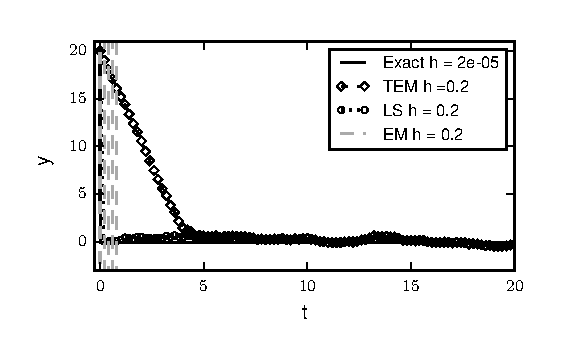
\includegraphics[width=\textwidth]{Imagenes/NumericalResults/ApplebyEx.eps}
%			}
%		\end{overlayarea}
%		\column{.4\textwidth}
%			\begin{overlayarea}{\textwidth}{\textheight}
%				\begin{bibunit}[apalike]
%					\nocite{Appleby2010}
%					\only<2->{
%						\biblio{PhdThesisBib}	
%					}
%				\end{bibunit}
%			\end{overlayarea}
%	\end{columns}	
%\end{frame}
%%%%%%%%%%%%%%%%%%%%%%%%%%%%%%%%%%%%%%%%%%%%%%%%%%%%%%%%%%%%%%%%%%%%%%%%%%%%%%%%%%%%%%%%%%%%%%%%%%%%%%%%
\begin{frame}
	\frametitle{EDE con difusi\'on superlineal}
	\begin{overlayarea}{\textwidth}{.2\textheight}
		\begin{empheq}[box=\shadowbox*]{equation*}
			dy(t) =
				\left(
					1-y^5(t) +y^3(t)  
				\right) dt
				+
			\textcolor{red}{
				y^2(t)
			}
			dW(t),
				 \qquad y_0=0
		\end{empheq}
	\end{overlayarea}
	%
	\begin{columns}
		\column{.6\textwidth}
		\begin{overlayarea}{\textwidth}{.8\textheight}
			\only<2>{
				\vspace{-1.8cm}
				\begin{align*}
					a(x)&:= -x^4 +x^2, \quad b: = 1 ,  \quad E=\{-1,0,1\}\\
					Y_{k+1}&= \exp(ha(Y_k))Y_k + 
						\frac{\exp(ha(Y_k)) - 1}{a(Y_k)} \1{E^c} \\
						&+h\1{E}+Y_k^2\Delta W_k. 	
				\end{align*}
			}
			\only<3->{
				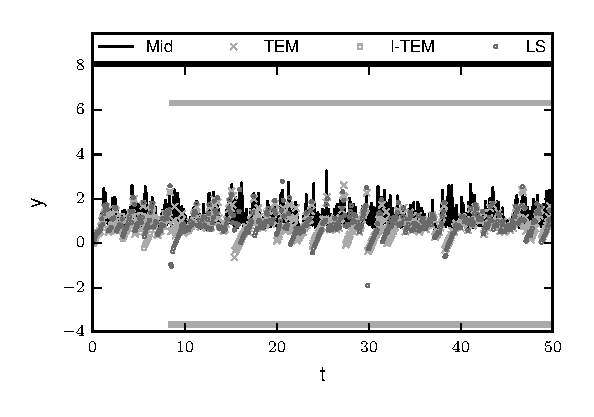
\includegraphics[width=\textwidth]{Imagenes/NumericalResults/Tretyakov.eps}
			}
		\end{overlayarea}
		\column{.4\textwidth}
		\begin{overlayarea}{\textwidth}{\textheight}
			\begin{bibunit}[apalike]
				\nocite{Tretyakov2013}
				\only<3->{
					\biblio{PhdThesisBib}	
				}
			\end{bibunit}
		\end{overlayarea}
	\end{columns}	
\end{frame}
%%%%%%%%%%%%%%%%%%%%%%%%%%%%%%%%%%%%%%%%%%%%%%%%%%%%%%%%%%%%%%%%%%%%%%%%%%%%%%%%%%%%%%%%%%%%%%%%%%%%%%%%
\begin{frame}
	\frametitle{Sistemas (Ecuaci\'on de Langevin)}
	\begin{empheq}[box={\Garybox[\scalebox{.6}{$U(x)= \frac{1}{4}|x|^4 - \frac{1}{2}|x|^2$}]}]{equation*}
		dy(t) = 
		\left(
		y(t) - |y(t)|^2 \cdot y(t)
		\right)dt
		+ dW(t), \quad y(0)=0
	\end{empheq}
	%
	\begin{columns}
		\column{.6\textwidth}
		\begin{overlayarea}{\textwidth}{.8\textheight}
			\only<2>{
				\hspace{-.5cm}
\scalebox{.7}{
%\centering
\begin{tabular}{lllllll}
	&        TEM &        	& LS		&           & BEM		 &         \\
	\toprule
	h		& ms-error	 & ECO 		& ms-error	    & ECO		& ms-error	 &	ECO	  \\
	\midrule
	$2^{-2}$	& \num{1.70388}    & ---		&\num{1.55394}		& ---		& \num{1.38157}	& 
	--- \\
	$2^{-3}$	& \num{1.16977}    & \num{0.54}     &\num{1.10775}    & \num{0.48} & \num{1.05309}	& 
	\num{0.39} \\ 
	$2^{-7}$	&\num{0.27895}     & \num{0.48} & \num{0.27795}   & \num{0.48} & \num{0.276895}& 
	\num{0.48} \\
	$2^{-11}$	& \num{0.07010}  & \num{0.50} & \num{0.07009}  & \num{0.50} & \num{0.07007} & 
	\num{0.50} \\
	$2^{-15}$	& \num{0.01739}  & \num{0.51} & \num{0.01739}  & \num{0.51} & \num{0.01739}& 
	\num{0.51} \\
	\bottomrule
\end{tabular}
}
			}
			\only<3->{
				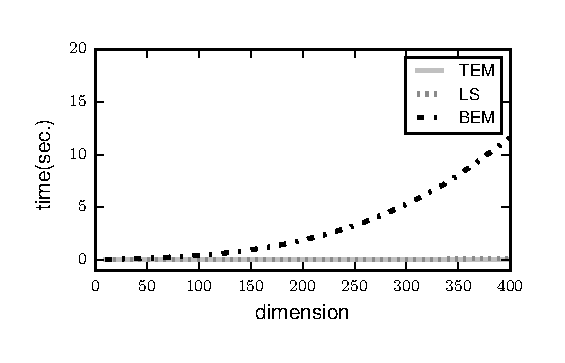
\includegraphics[width=\textwidth]{Imagenes/NumericalResults/TimeVsDimension.eps}
			}
		\end{overlayarea}
		\column{.4\textwidth}
		\begin{overlayarea}{\textwidth}{.8\textheight}
			\begin{bibunit}[apalike]
				\nocite{Hutzenthaler2012a}
				\only<2->{
					\biblio{PhdThesisBib}	
				}
			\end{bibunit}
		\end{overlayarea}
	\end{columns}	
\end{frame}
%%%%%%%%%%%%%%%%%%%%%%%%%%%%%%%%%%%%%%%%%%%%%%%%%%%%%%%%%%%%%%%%%%%%%%%%%%%%%%%%%%%%%%%%%%%%%%%%%%%%
\begin{frame}
	\frametitle{Contra ejemplo para los tamed}
	\vspace{2mm}
	\begin{tcolorbox}[size=tight]
		\scalebox{.98}{\parbox{\linewidth}
			{
			\begin{align*}
				dy_1(t) &=
					\left(
						\lambda -\delta y_1(t) - (1 - \gamma) \beta y_1(t) y_3(t)
					\right)dt
					-\sigma_1 y_1(t) dW^{(1)}_t, \notag \\
				dy_2(t) &= 	
					\left(
						(1- \gamma) \beta y_1(t) y_3(t) - \alpha y_2(t) 
					\right)dt
					-\sigma_1 y_2(t) dW^{(1)}_t, \\
				dy_3(t) & = 
					\left(
						(1 - \eta) N_0 \alpha y_2(t) 
						-\mu y_3(t)
						-(1 - \gamma ) \beta y_1(t) y_3(t) 
					\right)dt
					- \sigma_2 y_3(t) dW^{(2)}_t
			\end{align*}
			}
		}
	\end{tcolorbox}
%
	\begin{columns}
		\column{.7\textwidth}
		\begin{overlayarea}{\textwidth}{.8\textheight}
			\only<2->{
				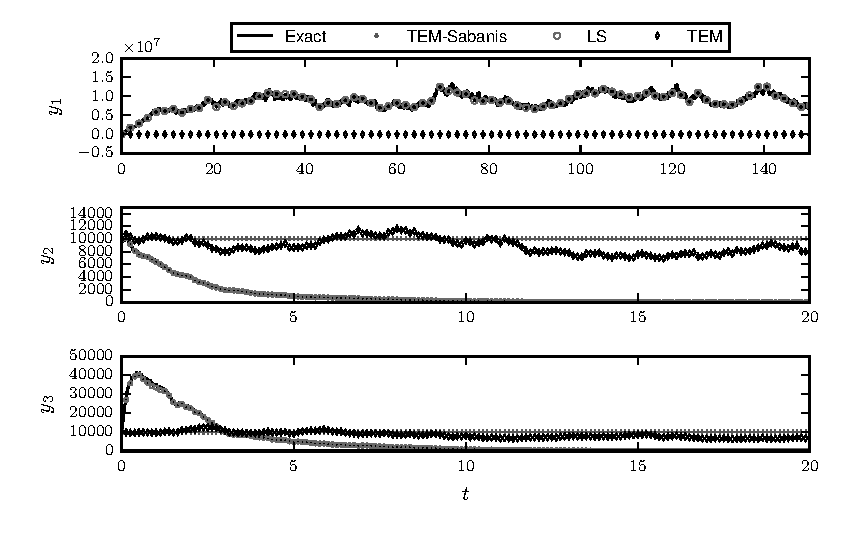
\includegraphics[width=\linewidth]{Imagenes/NumericalResults/InternalHIVDynamics.eps}
			}
		\end{overlayarea}
		\column{.4\textwidth}
		\begin{overlayarea}{\textwidth}{.8\textheight}
			\only<2>{
				$\gamma = \num{0.5}$,
				$\eta = \num{0.5}$,
				$\lambda = \num{e6}$, 
				$\delta = \num{0.1}$,
				$\beta = \num{e-8}$,
				$\alpha = \num{0.5}$,
				$N_0= \num{100}$,
				$\mu = \num{5}$,
				$\sigma_1 = \num{0.1}$,
				$\sigma_2 = \num{0.1} $,
				\\
				$y_0 = (
				\num{10000},%{\per\cubic\deci\meter}, 
				\num{10000},%{\per\cubic\deci\meter}, 
				\num{10000}.%{\per\cubic\deci\meter}
			)^T$,
				$h=\num{0.125}$.
				\\
				Exacta: BEM $h=\num{e-5}$
			}
			\begin{bibunit}[apalike]
				\nocite{Dalal2008}
				\only<3->{
					\biblio{PhdThesisBib}	
				}
			\end{bibunit}
		\end{overlayarea}
	\end{columns}	
\end{frame}
%%%%%%%%%%%%%%%%%%%%%%%%%%%%%%%%%%%%%%%%%%%%%%%%%%%%%%%%%%%%%%%%%%%%%%%%%%%%%%%%%%%%%%%%%%%%%%%%%%%%%%%%%
